La titolazione è una tipica operazione dell'analisi chimica che consiste nel determinare la concentrazione o \textbf{titolo} di una specie chimica in soluzione, facendola reagire con una quantità nota di un dato reagente, detto \textbf{titolante}.
\subsection{Titolazione acido forte-base forte}
Si versa in un becher dell'acido e si aggiungono una o al massimo due gocce di una soluzione di una specie chiamata \textit{indicatore}. L'indicatore è un composto che cambia colore nell'istante in cui si passa da un valore di pH ad un altro. Questo cambiamento di colore è chiamato \textit{viraggio dell'indicatore}.

Ci sono vari tipi di indicatori. Se volessimo osservare la fine della titolazione, ossia partiamo da una soluzione acida e aggiungiamo una base, è utile un indicatore che abbia un punto di viraggio per pH pari a 7. Non è necessario che l'indicatore cambi colore esattamente a quel pH, perché ci sarà un valore di pH acido superato il quale, con appena qualche goccia di base, si raggiunge l'equivalenza. Gli indicatori sono dunque delle sostanze che cambiano colore in modo visibile ai nostri occhi e forniscono indicazioni sul cambiamento di pH.

Nel caso specifico di questa reazione, conviene utilizzare come indicatore una sostanza chiamata \textit{fenoltaleina}, o meglio soluzioni estremamente diluite (all'1\%) di questa. Basta aggiungere una goccia di questa soluzione nel becher per poter osservare un cambio di colore quasi immediato. Quando?

\begin{figure}[H]
    \centering
    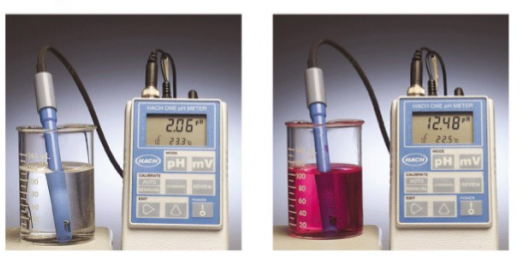
\includegraphics[width=14cm]{immagini/Fenoltaleina.png}
\end{figure}

In ambiente acido è incolore (quindi ad esempio partendo da una soluzione di acido cloridrico non vedremmo nulla), mentre per pH tra 8.5 e 9 da incolore diventa rossa, quindi avremo l'indicazione che il pH ha raggiunto tale valore al cambio di colore della soluzione. Se avessimo voluto capire invece quando si aveva l'equivalenza (cioè pH=7), potremmo pensare di aver perso questo punto di equivalenza. Vedremo che non è così: in prossimità del punto di equivalenza il pH varierà in modo repentino, con piccolissime aggiunte; al contrario, quando si è lontani dal punto di equivalenza il pH cambierà molto poco pur aggiungendo, se partiamo da una soluzione acida, parecchia base. D'altronde, avendo definito il pH come il logaritmo dell'inverso della concentrazione degli ioni $\rm H_3O^+$ di una soluzione, ci aspettiamo un andamento logaritmico e non lineare per il pH dopo l'aggiunta di una base.

\vspace{0.2cm}Immaginiamo di avere due soluzioni in due becher diversi. Nel primo abbiamo 100 mL di HCl 0.1 N (nota: per l'HCl normalità e molarità coincidono). Aggiungiamo in esso la prima goccia di indicatore e poi aggiungiamo lentamente NaOH 0.1 N\footnote{Ovviamente non è necessario scegliere stesse concentrazioni, le usiamo per comodità di calcolo.}. In questo caso, se partiamo da 100 mL di acido cloridrico 0.1 N, quando avremo aggiunto 100 mL di idrossido di sodio 0.1 N (quindi stessi volumi e stesse concentrazioni) non avremo più né acido né base perché si saranno neutralizzati totalmente formando cloruro di sodio:

$$\ce{HCl(aq) + NaOH(aq) -> NaCl(aq) + H_2O}$$

Va ricordato che HCl acquoso, visto che si tratta di un acido forte, significa ione $\rm H_3O^+$ e ione $\rm Cl^-$ totalmente dissociati. Analogamente NaOH acquoso, visto che si tratta di una base forte, significa ione $\rm Na^+$ e ione $\rm OH^-$ totalmente dissociati. Ma anche il cloruro di sodio, essendo un sale e quindi un elettrolita forte, sarà totalmente dissociato in $\rm Na^+$ e $\rm Cl^-$. Ne segue che l'unica vera reazione che sta venendo è la formazione di acqua: lo ione $\rm H^+$ dell'acido cloridrico e lo ione $\rm OH^-$ dell'NaOH danno luogo ad $\rm H_2O$, mentre gli altri ioni restano dissociati prima e dopo la reazione.

Quant'è il pH della soluzione iniziale?

Inizialmente abbiamo solo acido cloridrico. Scriviamo sopra la reazione le quantità iniziali, sotto quelle finali:

\begin{center}
    \begin{tabular}{ccccccc}
        0.01 &  & / & & / & &\\
        HCl & + & NaOH & \ce{->} & NaCl & + & $\rm H_2O$\\
        0.01 &  &  / & & / & &\\
    \end{tabular}
\end{center}

(Non c'è base con cui reagire, quindi le moli finali sono uguali a quelle iniziali)

All'inizio abbiamo 100 mL di HCl 0.1 N, il che significa (in questo caso in cui moli ed equivalenti coincidono) 0.1 moli in un litro di soluzione, quindi per sapere quante moli ( o equivalenti) abbiamo in 1 mL dobbiamo dividere per 1000.

Per sapere gli equivalenti totali dobbiamo fare

$$\frac{0.1}{1000} \cdot 100$$

Per avere il pH prima di aggiungere base non è necessario nemmeno questo calcolo perché abbiamo già la concentrazione. Infatti il pH è definito come

$$\rm pH=\log \frac{1}{[H_3O^+]}$$

Ricordiamo che l'acido cloridrico in acqua darà luogo a ioni $\rm H_3O^+$ e ioni $\rm Cl^-$:

$$\ce{HCl + H_2O -> H_3O^+ + Cl^-}$$

Essendo un acido forte, tale reazione è compiuta da tutto l'acido. Ne segue che la concentrazione degli ioni $\rm H_3O^+$ corrisponde alla concentrazione dell'acido cloridrico.

$\rm [H_3O^+]$ è espressa come equivalenti/litro, che abbiamo già. Quindi il pH sarà

$$\rm pH=\log\frac{1}{0.1}=\log10=1$$

Quindi ancora prima di iniziare l'aggiunta della base abbiamo una soluzione che ha pH pari a 1.

A questo punto facciamo la prima aggiunta. Queste vanno fatte lentamente, quindi inizialmente aggiungiamo 10 mL di base. Dopo averli aggiunti calcoliamo il pH.

Torniamo alla reazione. Gli equivalenti iniziali di HCl erano 0.01 eq. Quanti equivalenti (o moli) ci sono in 10 mL di base? Il calcolo è lo stesso:

$$\frac{0.1}{1000} \cdot 10=10^{-3}=0.001 \; eq$$

Quindi, dopo la prima aggiunta e prima della reazione, abbiamo 0.01 eq di HCl e 0.001 eq di NaOH. Ci accorgiamo che quest'ultimo è in difetto, quindi sarà tutto consumato per produrre cloruro di sodio. Ne segue che avremo $10^{-3}$ moli di NaCl, mentre di HCl ne resterà la differenza, cioè $9 \cdot 10^{-3}$ moli.

Schematizzando, i valori prima e dopo saranno

\begin{center}
    \begin{tabular}{ccccccc}
        0.01 &  & 0.001 & & / & &\\
        HCl & + & NaOH & \ce{->} & NaCl & + & $\rm H_2O$\\
        0.009 &  &  / & & 0.001 & &\\
    \end{tabular}
\end{center}

Calcoliamo la concentrazione di questa soluzione.

Non abbiamo base, abbiamo solo l'acido di cui ci sono $9 \cdot 10^{-3}$ moli. Esse stanno in un volume di 110 mL, quindi la molarità (e dunque la normalità) sarà data da

$$M=9 \cdot 10^{-3} \, \frac{1000}{110}=8.1818 \cdot 10^{-2}$$

Questa è la molarità della soluzione acida, perché la base è scomparsa e abbiamo solo acido cloridrico. Il calcolo da fare sarà allora

$$\rm pH=\log\left( \frac{1}{8.1818 \cdot 10^{-2}} \right)=1.09$$

A questo punto aggiungiamo 20 mL di NaOH, considerando però la quantità di acido di partenza.

Calcoliamo le moli di NaOH

$$n=\frac{0.1}{1000}\cdot 20=2 \cdot 10^{-3}$$

L'NaOH è in difetto e formerà 0.002 moli di sale. Di acido ce ne rimangono 0.008 moli

\begin{center}
    \begin{tabular}{ccccccc}
        0.01 &  & 0.002 & & / & &\\
        HCl & + & NaOH & \ce{->} & NaCl & + & $\rm H_2O$\\
        0.008 &  &  / & & 0.002 & &\\
    \end{tabular}
\end{center}

La molarità sarà

$$M=8\cdot 10^{-3} \, \frac{1000}{120}=6.6667 \cdot 10^{-2}$$

La soluzione è ancora acida, pertanto

$$\rm pH=\log\left( \frac{1}{6.6667 \cdot 10^{-2}} \right)=1.18$$

Adesso aggiungiamo 40 mL di base. Le moli di NaOH saranno $4 \cdot 10^{-3}$ (calcolate come prima), per cui la base continua ad essere in difetto, quindi viene neutralizzata totalmente, dando $4 \cdot 10^{-3}$ moli di sale. Ci restano 0.006 moli di acido:

\begin{center}
    \begin{tabular}{ccccccc}
        0.01 &  & 0.004 & & / & &\\
        HCl & + & NaOH & \ce{->} & NaCl & + & $\rm H_2O$\\
        0.006 &  &  / & & 0.004 & &\\
    \end{tabular}
\end{center}

La molarità sarà

$$M=6\cdot 10^{-3} \, \frac{1000}{140}=4.2857\cdot 10^{-2}$$

$$\implies \rm pH=\log\left( \frac{1}{4.2857 \cdot 10^{-2}} \right)=1.37$$

Aggiungiamo 50 mL di NaOH 0.1 N. A questo punto arriviamo a metà della titolazione. Si ottengono 0.005 moli di sale e restano 0.005 moli di acido

\begin{center}
    \begin{tabular}{ccccccc}
        0.01 &  & 0.005 & & / & &\\
        HCl & + & NaOH & \ce{->} & NaCl & + & $\rm H_2O$\\
        0.005 &  &  / & & 0.005 & &\\
    \end{tabular}
\end{center}

$$M=5 \cdot 10^{-3} \, \frac{1000}{150}=3.333 \cdot 10^{-2}$$

$$\implies \rm pH = \log \left( \frac{1}{3.333 \cdot 10^{-2}} \right)=1.48$$

Notiamo che, pur avendo neutralizzato metà dell'acido di partenza, il pH non è aumentato nemmeno di mezza unità.

\vspace{0.2cm}Calcoliamo il pH dopo aver aggiunto 80 mL di base.

Abbiamo aggiunto 0.008 equivalenti (o moli) di base, che sono ancora in difetto, quindi vanno via producendo 0.008 moli di sale e ci restano 0.002 moli di acido:

\begin{center}
    \begin{tabular}{ccccccc}
        0.01 &  & 0.008 & & / & &\\
        HCl & + & NaOH & \ce{->} & NaCl & + & $\rm H_2O$\\
        0.002 &  &  / & & 0.008 & &\\
    \end{tabular}
\end{center}

La molarità dell'acido sarà

$$M=2 \cdot 10^{-3} \, \frac{1000}{180}=1.1111 \cdot 10^{-2}$$

$$\implies \rm pH = \log \left( \frac{1}{1.1111 \cdot 10^{-2}} \right)=1.95$$


Aggiungiamo 90 mL di base, che significa 0.009 moli. Essendo in difetto, l'NaOH va tutto via e dà 0.009 moli di sale e restano 0.001 moli di acido:

\begin{center}
    \begin{tabular}{ccccccc}
        0.01 &  & 0.009 & & / & &\\
        HCl & + & NaOH & \ce{->} & NaCl & + & $\rm H_2O$\\
        0.001 &  &  / & & 0.009 & &\\
    \end{tabular}
\end{center}

La concentrazione è

$$M=1 \cdot 10^{-3} \, \frac{1000}{190}=5.2632 \cdot 10^{-3}$$

$$\implies \rm pH = \log \left( \frac{1}{5.2632 \cdot 10^{-3}} \right)=2.28$$

Aggiungiamo adesso 95 mL, cioè $9.5 \cdot 10^{-3}$ moli di base, che sono in difetto e producono $9.5 \cdot 10^{-3}$ moli di sale. Restano $5 \cdot 10^{-4}$ moli di acido.

\begin{center}
    \begin{tabular}{ccccccc}
        0.01 &  & $9.5 \cdot 10^{-3}$  & & / & &\\
        HCl & + & NaOH & \ce{->} & NaCl & + & $\rm H_2O$\\
        $5 \cdot 10^{-4}$ &  &  / & & $9.5 \cdot 10^{-3}$ & &\\
    \end{tabular}
\end{center}

$$M=5 \cdot 10^{-4} \, \frac{1000}{195}=2.5641 \cdot 10^{-3}$$

$$\implies \rm pH=\log \left( \frac{1}{2.5641 \cdot 10^{-3}} \right)=2.59$$

Andiamo a 99 mL. Avremo $9.9 \cdot 10^{-3}$ moli di base e quindi $1.0 \cdot 10^{-4}$ moli di acido

\begin{center}
    \begin{tabular}{ccccccc}
        0.01 &  & $9.9 \cdot 10^{-3}$  & & / & &\\
        HCl & + & NaOH & \ce{->} & NaCl & + & $\rm H_2O$\\
        $1 \cdot 10^{-4}$ &  &  / & & $9.9 \cdot 10^{-3}$ & &\\
    \end{tabular}
\end{center}

$$M=1.0 \cdot 10^{-4} \, \frac{1000}{199}=5.0251\cdot 10^{-4}$$

$$\implies \rm pH=\log \left( \frac{1}{5.0251\cdot 10^{-4}} \right)=3.30$$

Aggiungiamo 99.5 mL. Le moli di base saranno $9.95 \cdot 10^{-3}$. Siamo ancora in difetto, quindi avremo $9.95 \cdot 10^{-3}$ moli di sale e restano $5 \cdot 10^{-5}$ moli di acido

\begin{center}
    \begin{tabular}{ccccccc}
        0.01 &  & $9.95 \cdot 10^{-3}$  & & / & &\\
        HCl & + & NaOH & \ce{->} & NaCl & + & $\rm H_2O$\\
        $5 \cdot 10^{-5}$ &  &  / & & $9.95 \cdot 10^{-3}$ & &\\
    \end{tabular}
\end{center}

$$M=5.0 \cdot 10^{-5} \, \frac{1000}{199.5}=2.5063 \cdot 10^{-4}$$

$$\implies \rm pH=\log \left( \frac{1}{2.5063 \cdot 10^{-4}} \right)=3.60$$

Aggiungiamo 99.9 mL. Le moli di base saranno $9.99 \cdot 10^{-3}$. La base continua ad essere in difetto e produrrà $9.99 \cdot 10^{-3}$ moli di sale. Resteranno $1 \cdot 10^{-5}$ moli di acido

\begin{center}
    \begin{tabular}{ccccccc}
        0.01 &  & $9.99 \cdot 10^{-3}$  & & / & &\\
        HCl & + & NaOH & \ce{->} & NaCl & + & $\rm H_2O$\\
        $1 \cdot 10^{-5}$ &  &  / & & $9.99 \cdot 10^{-3}$ & &\\
    \end{tabular}
\end{center}

$$M=1 \cdot 10^{-5} \, \frac{1000}{199.9}=5.0025 \cdot 10^{-5}$$

$$\implies \rm pH=\log \left( \frac{1}{5.0025 \cdot 10^{-5}} \right)=4.30$$

Gli strumenti che usiamo per aggiungere la base si chiamano burette. Esse hanno la precisione di 0.1 mL. Il loro rubinetto può però essere aperto in modo tale da fare scendere la soluzione goccia a goccia e le burette sono tali che 1 mL contenga 20 gocce. Una goccia quindi contiene 1/20 di mL, ossia il volume di una goccia è 0.05 mL.

Aggiungiamo quindi come volume della base 99.95 mL. Avremo $9.995 \cdot 10^{-3}$ moli di base e quindi anche di sale perché non abbiamo eccesso di base. Restano poi $5 \cdot 10^{-6}$ moli di acido:

\begin{center}
    \begin{tabular}{ccccccc}
        0.01 &  & $9.995 \cdot 10^{-3}$  & & / & &\\
        HCl & + & NaOH & \ce{->} & NaCl & + & $\rm H_2O$\\
        $5 \cdot 10^{-6}$ &  &  / & & $9.995 \cdot 10^{-3}$ & &\\
    \end{tabular}
\end{center}

$$M=5 \cdot 10^{-6} \, \frac{1000}{199.95}=2.5006 \cdot 10^{-5}$$

$$\implies \rm pH=\log \left( \frac{1}{2.5006 \cdot 10^{-5}} \right)=4.60$$

Ci resta l'ultima goccia per la neutralizzazione totale, cioè aggiungiamo 100 mL di base

\begin{center}
    \begin{tabular}{ccccccc}
        0.01 &  & 0.01  & & / & &\\
        HCl & + & NaOH & \ce{->} & NaCl & + & $\rm H_2O$\\
        / &  & / & & 0.01 & &\\
    \end{tabular}
\end{center}

A questo punto la concentrazione degli ioni $\rm H_3O^+$, ossia la molarità, qual è? Non abbiamo più né acido né base e il cloruro di sodio è un sale neutro, pertanto sarà quella dell'autodissociazione dell'acqua:

$$\rm [H_3O^+]=10^{-7} \implies pH=7$$

A questo punto riportiamo i valori del pH e dei mL di base in una tabella:

\begin{center}
    \begin{tabular}{|p{1.5cm}|p{1.5cm}||p{1.5cm}|p{1.5cm}|}
        \textbf{pH} & \textbf{mL} & \textbf{pH} & \textbf{mL}\\
        1 & 0 & 2.59 & 95\\
        1.09 & 10 & 3.30 & 99\\
        1.18 & 20 & 3.60 & 99.5\\
        1.37 & 40 & 4.30 & 99.9\\
        1.48 & 50 & 4.60 & 99.95\\
        1.95 & 80 & 7 & 100\\
        2.28 & 90 &&\\
    \end{tabular}
\end{center}

Notiamo che all'inizio il pH cambiava pochissimo: 10 mL fanno variare il pH di meno di 0.1; 20 mL di meno di 0.2; 40 mL di meno di 0.4 e 50 mL meno di 0.5. Quando siamo arrivati a 90 mL abbiamo superato il valore di 2, perché con 80 mL il pH valeva ancora 1.95. Tra 95 mL e 99 mL, cioè 4 mL in più, il pH cambia da 2.28 a 2.59, infatti ci stiamo avvicinando alla salita logaritmica. Infine quando mancano due gocce alla neutralità il pH è 4.30, quando ne manca solamente una il pH è 4.60 e dopo avere aggiunto pure l'ultima goccia il pH è 7.

Notiamo che serve molta precisione, quindi conviene usare 4 cifre dopo la virgola approssimando la quarta cifra dopo aver letto la quinta.

Continuiamo: aggiungiamo un'ulteriore goccia, quindi si hanno 100.05 mL di base, ossia una goccia in più rispetto alla neutralità. Avremo $(0.1 \cdot 100.05)/1000=1.0005 \cdot 10^{-2}$ moli di base, che è in eccesso. Quindi stavolta l'acido cloridrico va via del tutto e produce 0.01 moli di sale. Restano $5 \cdot 10^{-6}$ moli di base:

\begin{center}
    \begin{tabular}{ccccccc}
        0.01 &  & $1.0005 \cdot 10^{-2}$ & & / & &\\
        HCl & + & NaOH & \ce{->} & NaCl & + & $\rm H_2O$\\
        / &  &  $5 \cdot 10^{-6}$ & & 0.01 & &\\
    \end{tabular}
\end{center}

La molarità sarà, calcolata rispetto all'NaOH:

$$M=5 \cdot 10^{-6} \, \frac{1000}{200.5}=2.4993 \cdot 10^{-5}$$

Avendo una base dobbiamo calcolare il pOH:

$$\rm pOH = \log \left( \frac{1}{2.4993 \cdot 10^{-5}} \right)=4.6$$

$$\implies \rm pH=14 - pOH=14-4.6=9.40$$

\E da notare che con due gocce abbiamo avuto un salto di 6 unità di pH, ciò perché siamo in prossimità dell'equivalenza. Infatti lontano da essa sono serviti 90 mL di base per portare il pH da 1 a 2, qua invece abbiamo usato solo 0.1 mL.

Aggiungiamo un'altra goccia di base, cioè 100.1 mL di base

$$n_{\text{NaOH}}=\frac{0.1 \cdot 100.1}{1000}\approx 0.01001\implies n_{\text{residue}}=0.01001-0.01 = 1 \cdot 10^{-5}$$

$$M=1 \cdot 10^{-5} \, \frac{1000}{200.1}=4.9975 \cdot 10^{-5}$$

$$\rm pOH=\log \left( \frac{1}{4.9975 \cdot 10^{-5}} \right)=4.30 \implies \rm pH=14-4.30=9.70$$

Aggiungiamo 110 mL di titolante

$$n_{\text{NaOH}}=\frac{0.1 \cdot 110}{1000}= 0.011\implies n_{\text{residue}}=0.011-0.01 = 1 \cdot 10^{-3}$$

$$M=1 \cdot 10^{-3} \, \frac{1000}{210}=4.7619 \cdot 10^{-3}$$

$$\rm pOH=\log \left( \frac{1}{4.7619 \cdot 10^{-3}} \right)=2.32 \implies \rm pH=14-2.32=11.67$$

Aggiungiamo 120 mL di titolante

$$n_{\text{NaOH}}=\frac{0.1 \cdot 120}{1000}= 0.012\implies n_{\text{residue}}=0.012-0.01 = 2 \cdot 10^{-3}$$

$$M=2 \cdot 10^{-3} \, \frac{1000}{220}=9.0909 \cdot 10^{-3}$$

$$\rm pOH=\log \left( \frac{1}{9.0909 \cdot 10^{-3}} \right)=2.04 \implies \rm pH=14-2.04=11.96$$

Aggiungiamo 150 mL di titolante

$$n_{\text{NaOH}}=\frac{0.1 \cdot 150}{1000}= 0.015\implies n_{\text{residue}}=0.015-0.01 = 5 \cdot 10^{-3}$$

$$M=5 \cdot 10^{-3} \, \frac{1000}{250}=2 \cdot 10^{-2}$$

$$\rm pOH=\log \left( \frac{1}{2 \cdot 10^{-2}} \right)=1.69 \implies \rm pH=14-1.69=12.31$$

Se riportiamo i dati su un grafico avremo tale andamento:

\begin{figure}[H]
    \hspace{1.3cm}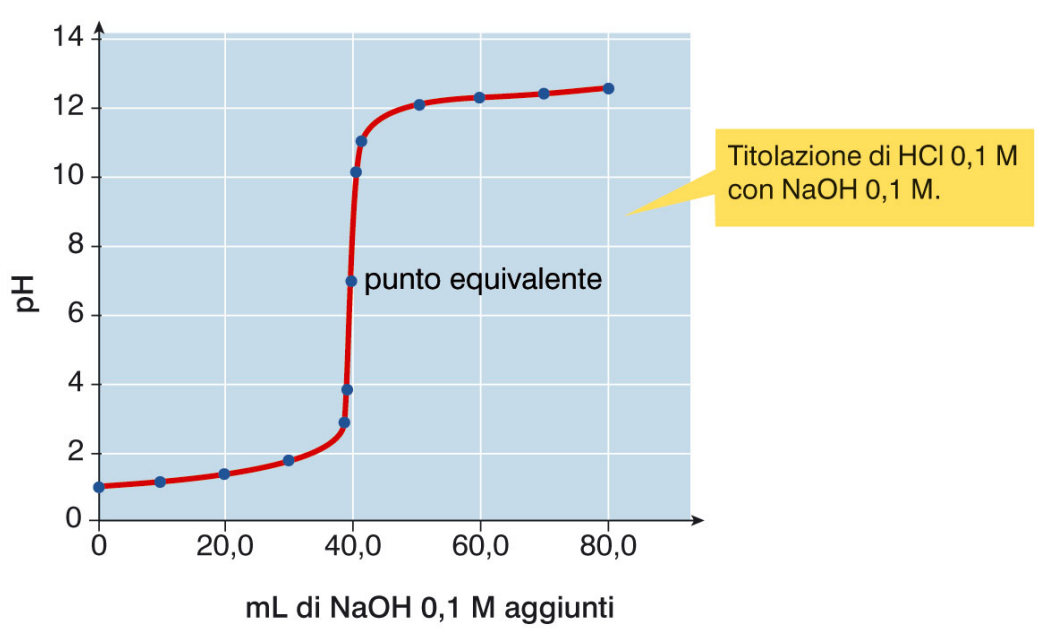
\includegraphics[width=14cm]{immagini/titolazione_acido_forte_base_forte.png}
\end{figure}

Per questa titolazione acido forte-base forte si ha il flesso per pH=7.

Se fossimo partiti al contrario da una base e avessimo aggiunto l'acido, il pH sarebbe stato alto all'inizio, variando inizialmente poco e bruscamente poi in prossimità dell'equivalenza per poi appiattirsi di nuovo.

A questo punto capiamo che qualunque indicatore abbia un intervallo di viraggio compreso nella regione in cui il pH varia velocemente è ottimo per i nostri scopi, perché avremo variazione di pH con poche gocce. Se inoltre sappiamo a priori quando l'indicatore vira (ad esempio la fenoltaleina vira tra 8.8 e 9), possiamo capire di quanto abbiamo ecceduto nell'aggiungere il titolante. Chiaramente bisogna essere pronti a chiudere il rubinetto appena vediamo la soluzione cambiare colore.

Sapendo quando l'indicatore vira possiamo capire quante gocce dobbiamo aggiungere o togliere per arrivare a pH pari a 7.

Affinché l'indicatore sia utile ai nostri scopi serve che il suo intervallo di viraggio sia nell'arco di 1-2 gocce.

A cosa serve questo discorso?

Se avessimo delle soluzioni di cui conosciamo precisamente la concentrazione questo lavoro non servirebbe. Se invece avessimo una soluzione di una data specie di cui non conosciamo la concentrazione, con questo metodo potremmo ottenerla, perché ciò che succede è che abbiamo un becher in cui c'è una certa quantità di una specie (acido o base che sia) e poi ne aggiungiamo un'altra, quindi conosciamo con esattezza i due volumi, quello della specie nel becher e quello che misuriamo goccia a goccia. Avremo la neutralità quando gli ioni $\rm H_3O^+$ provengono esclusivamente dall'autodissociazione dell'acqua, ossia quando l'acido e la base che abbiamo aggiunto sono esattamente uguali in moli. Non appena il numero di moli è uguale a meno di una goccia, l'indicatore vira, facendo cambiare colore alla soluzione e indicandoci di fermarci.

In questa condizione valgono le espressioni

$$N_1V_1=N_2V_2
\quad
;
\quad
M_1V_1=M_2V_2$$

dove $N$ è la normalità e $M$ la molarità. Entrambe sono espressioni per indicare il numero di moli.

Immaginiamo di avere dell'acido cloridrico a concentrazione $M_1$ incognita. Di esso ne preleviamo un volume $V_1$ a piacere. (Attenzione! Nell'esempio la concentrazione la abbiamo, ci è stata data solo per fare meno calcoli). Andiamo allora a prendere dell'NaOH della quale sia nota la concentrazione e di cui quindi conosciamo la molarità $M_2$, ed iniziamo ad aggiungere pian piano il volume $V_2$ fino a quando la soluzione in cui è messo l'indicatore cambia colore; in quel momento chiudiamo il rubinetto e leggiamo il volume di NaOH aggiunto e andiamo a calcolare $M_1$.

\vspace{0.2cm}Quindi abbiamo usato questo metodo per più motivi:

\begin{itemize}
    \item Avere percezione di come vari il pH per aggiunte di una specie forte ad un'altra forte (cioè un acido o una base o viceversa);
    \item Capire quanto possiamo andare spediti nell'aggiungere il volume di titolante. Se avessimo poi già una stima di quella che è la concentrazione della specie che era nel becher, faremo attenzione arrivati al punto di viraggio aggiungendo una goccia ogni 5-10 secondi;
    \item Capire la sensibilità della scala del pH.
\end{itemize}

\subsection{Acidi deboli}
Come calcoliamo il pH di una specie che invece non è forte, cioè una specie di cui ne mettiamo una certa quantità ma se ne dissocia poca?

Nella reazione tra HCl e NaOH abbiamo utilizzato un criterio: la concentrazione degli ioni $\rm H_3O^+$ è uguale a quella dell'HCl in eccesso (o se eravamo a destra dell'equivalenza si assumeva la concentrazione degli ioni $\rm OH^-$ uguale a quella dell'NaOH in eccesso). Ciò non è più vero con un acido debole. L'esempio tipico è l'acido acetico:

$$\ce{CH_3COOH(aq) + H_2O <--> CH_3COO^-(aq) + H_3O^+(aq)}$$

L'acido acetico si dissocia poco, quindi avremo una reazione di equilibrio. La costante di questa dissociazione vale $1.8 \cdot 10^{-5}$, che per definizione si esprime come

$$k_a=\frac{\rm{[CH_3COO^-]} \cdot \rm{[H_3O^+]}}{\rm{[CH_3COOH]}}$$

Dal basso valore della costante deduciamo che si dissocia poco, ma quelle poche molecole che si dissociano producono uno ione acetato e uno ione $\rm H_3O^+$ ciascuna, quindi numericamente le due concentrazioni saranno sempre uguali. La costante si può allora scrivere come

$$k_a=\frac{\rm{[H_3O^+]^2}}{\rm{[CH_3COOH]}}$$

Nota: queste sono le quantità all'equilibrio, non quelle di partenza. Ne segue che al denominatore abbiamo la concentrazione dell'acido acetico rimasto.

 %Quindi se approssimiamo la concentrazione all'equilibrio come approssimativamente uguale a quella iniziale,

 Dunque nella dissociazione dell'acido acetico in acqua, la quantità di acido che si dissocia è estremamente piccola. Poiché il pH è dato con due cifre decimali, possiamo approssimare la concentrazione all'equilibrio con quella di partenza. Tale approssimazione ci evita un'equazione di secondo grado. Se infatti all'inizio avessimo ad esempio una mole di acido di cui se ne dissocia una quantità $x$, avremo $x$ moli di ione acetato e $x$ moli di $\rm H_3O^+$. Di acido ce ne restano $1-x$ moli:

\begin{center}
    \begin{tabular}{ccccccc}
        1 &  &  & & / & &\\
        $\rm CH_3COOH(aq)$ & + & $\rm H_2O$ & \ce{<-->} & $\rm CH_3COO^-(aq)$ & + & $\rm H_3O^+$\\
        $1-x$ & & & & $x$ & & $x$\\
    \end{tabular}
\end{center}

La costante allora diverrebbe $\displaystyle k=\frac{x^2}{1-x}$. Se invece partiamo da $c$ moli avremo

$$k_a = \frac{x^2}{c-x}$$%= \frac{x^2}{c-x}$$

Se però trascuriamo $x$ al denominatore avremo

$$[\text{H}_3\text{O}^+]^2= k_a \cdot c_a \implies [\text{H}_3\text{O}^+] = \sqrt{k_a \cdot c_a}$$

con $c_a$ concentrazione iniziale dell'acido.

Quindi la concentrazione degli ioni $\rm H_3O^+$ è data dalla radice della costante di equilibrio dell'acido per la sua concentrazione. Ciò non avviene per gli acidi forti in cui la concentrazione dell'acido coincide con quella degli ioni $\rm H_3O^+$.

Facciamo un esempio di calcolo: immaginiamo di avere 0.12345 grammi di $\rm CH_3COOH$ sciolti in una soluzione di 500 mL. Calcoliamo innanzitutto la concentrazione: anche quest'acido è monoprotico, quindi normalità e molarità coincidono perché peso molecolare e peso equivalente coincidono, per cui

$$c_a=N=M=\frac{0.12345 \cdot 1000}{60.052 \cdot 500}$$

$$\implies [\text{H}_3\text{O}^+]=\sqrt{1.8 \cdot 10^{-5} \cdot \frac{0.12345 \cdot 1000}{60.052 \cdot 500}}=2.7204 \cdot 10^{-4}$$

$$\implies \rm pH=\log \left( \frac{1}{2.7204 \cdot 10^{-4}} \right)=3.57$$

Gli acidi deboli, a parità di concentrazione con un acido forte, danno un pH meno acido. 

\subsection{Basi deboli}

L'esempio classico di pH di basi deboli è il caso dell'ammoniaca $\rm NH_3$, che è un gas. Noi lavoriamo con le soluzioni ammoniacali, cioè facciamo gorgogliare questo gas disciogliendolo in acqua. Quello che succede è che si forma l'addotto $\rm NH_3 \cdot H_2O$, cioè ogni molecola di $\rm NH_3$ associa una molecola d'acqua. A volte si fa la somma algebrica e si scrive $\rm NH_4OH$, ma è meno corretta. Ciononostante si usa perché ci dà un'idea più diretta della dissociazione che avviene:

$$\ce{NH_4OH <--> NH_4^+ + OH^-}$$

Useremo la prima notazione:

$$\ce{NH_3 \cdot H_2O <--> NH_4^+ + OH^-}$$

Questa sarà la dissociazione di tale base debole. La relativa costante di dissociazione è

$$k_b= \frac{\rm{[NH_4^+] \cdot [OH^-]}}{\rm{[NH_3 \cdot H_2O]}}$$

Quanto detto per l'acido acetico vale anche per questa base: ogni molecola di ammoniaca che si dissocia produrrà uno ione ammonio $\rm NH_4^+$ e uno ione $\rm OH^-$, quindi le loro concentrazioni saranno numericamente sempre uguali, quindi ci basta prenderne una ed elevarla al quadrato:

$$k_b= \frac{\rm{[OH^-]^2}}{\rm{[NH_3 \cdot H_2O]}}$$

$$\implies \rm [OH^-] = \sqrt{ \textit{k}_{\textit{b}} \cdot [NH_3 \cdot H_2O]}$$

La costante di dissociazione dell'$\rm NH_3$ è pari a $1.8 \cdot 10^{-5}$, ciò significa che questa dissociazione ha un equilibrio spostato a sinistra, ossia l'ammoniaca si dissocia poco. Pertanto possiamo trascurare la quantità che si è dissociata e immaginare che all'equilibrio si abbia la concentrazione iniziale della base:

$$[\text{OH}^-] = \sqrt{ k_b \cdot c_b}$$

In questo modo calcoliamo prima la concentrazione degli ioni $\rm OH^-$, poi il pOH e quindi il pH.

\vspace{0.2cm}Facciamo un esempio numerico: immaginiamo di avere 25 grammi di $\rm NH_3$ in un volume di 1 litro di soluzione finale. Attenzione! avremo 25 grammi della specie $\rm NH_3H_2O$, quindi il peso molecolare sarà circa 35. Dunque

$$[\text{OH}^-]=\sqrt{1.8 \cdot 10^{-5} \cdot \frac{25}{35}}=3.5857 \cdot 10^{-3}$$

$$\implies \rm pOH= \log \left( \frac{1}{3.5857 \cdot 10^{-3}} \right)=2.45 \implies pH=11.55$$

Abbiamo quindi visto che un'acido forte mostra un pH intorno ad 1, un acido debole un pH intorno a 3 (differenza notevole perché abbiamo a che fare con una scala logaritmica). Una base debole mostra pH superiore a 11. Tuttavia osservando le espressioni per acidi e basi deboli intuiamo che le concentrazioni sono fortemente determinate dalla costante di dissociazione. Ne segue che il pH delle specie deboli è fortemente determinato dalla costante. Facciamo questo confronto perché se avessimo la necessità di ottenere una soluzione con un dato pH dobbiamo sapere qual è la specie in grado di produrci tale pH, e per fare ciò si va a vedere il valore della costante di dissociazione.

\subsection{Reazioni di idrolisi}
Se mettiamo un cucchiaino di cloruro di sodio in acqua ciò che avviene è solo la dissociazione dell'NaCl in ione $\rm Na^+$ e $\rm Cl^-$, senza che questi subiscano reazioni successive:

$$\ce{NaCl(aq) -> Na^+(aq) + Cl^-(aq)}$$

Se anziché avere cloruro di sodio avessimo acetato di sodio $\rm CH_3COONa$ cosa succederebbe?

Questo composto in acqua si dissocia in ione acetato $\rm CH_3COO^-$ e ione $\rm Na^+$

$$\ce{CH_3COONa -> CH_3COO^-(aq) + Na^+(aq)}$$

Nota: mettiamo una singola freccia perché è un sale, e i sali solubili sono tutti elettroliti forti e pertanto totalmente dissociati.

Lo ione $\rm Na^+(aq)$ non darà luogo ad ulteriori reazioni perché in acqua si hanno ioni $\rm H_3O^+$ e ioni $\rm OH^-$. La specie NaOH non si potrà formare perché è una base forte quindi totalmente dissociata, cosa che porta lo ione $\rm Na^+$ e lo ione $\rm OH^-$ a non potersi riassociare.

Lo ione acetato $\rm CH_3COO^-$ invece è la base di un acido debole, per cui dà ulteriori reazioni. In particolare esso reagisce con una molecola d'acqua e dà un equilibrio (a differenza della prima reazione che è una dissociazione in cui non c'è equilibrio). Con tale reazione di equilibrio lo ione acetato strappa un protone all'acqua riformando l'acido acetico e lasciando ioni $\rm OH^-$

$$\ce{CH_3COO^-(aq) + H_2O <--> CH_3COOH(aq) + OH^-(aq)}$$

Si forma quindi un acido, ma la soluzione è basica. Queste reazioni sono dette di \textbf{idrolisi}, in particolare la reazione appena vista è detta \textbf{idrolisi basica}.

La soluzione sarà basica perché l'acido che si forma è indissociato, ma in soluzione abbiamo anche eccesso di ioni $\rm OH^-$.

Quello che sta succedendo è che mettiamo in acqua un sale che è neutro (l'acetato di sodio) e troviamo una soluzione che è basica. Questo discorso è tipico di tantissimi saponi: essi sono neutri finché sono lontani dall'acqua, ma appena li bagniamo la specie che si ottiene non è più neutra.

In sintesi: abbiamo messo in acqua un sale neutro, che essendo un elettrolita forte si dissocia totalmente, dando ione acetato e ione sodio. Quest'ultimo non fa nulla, resta $\rm Na^+(aq)$, ossia anche se ci sono ioni $\rm OH^-$ in soluzione non si avrà la formazione dell'NaOH perché quest'ultimo è una base forte, quindi è tutta dissociata e non può associarsi. Invece lo ione acetato che produciamo, che è la base coniugata di un acido debole, strappa un protone all'acqua, forma l'acido acetico e pertanto avremo un eccesso di ioni $\rm OH^-$.

Trattandosi di un equilibrio, scriviamo la costante di questo equilibrio $k_i$, che sta per \textit{costante di idrolisi}. In realtà potremmo scrivere $k_b$ perché abbiamo scoperto che l'acetato di sodio è una base, in quanto sviluppa un ambiente basico con eccesso di ioni $\rm OH^-$:

$$k_i = \rm{\frac{[CH_3COOH] [OH^-]}{[CH_3COO^-]}} \quad (*)$$

Tuttavia i testi non riportano questa costante, ma quella $k_a$ dell'acido acetico sì. Allora moltiplichiamo e dividiamo per la concentrazione degli ioni $\rm H_3O^+$:

$$k_i = \rm{\frac{[CH_3COOH] [OH^-]}{[CH_3COO^-]} \cdot \frac{[H_3O^+]}{[H_3O^+]}}$$

In tale espressione al numeratore compare il prodotto $\rm [OH^-] \cdot [H_3O^+]$, che è il prodotto ionico dell'acqua $k_w$ che vale $1.0 \cdot 10^{-14}$. Ciò che invece resta è uguale all'inverso della $k_a$ dell'acido acetico:

$$k_i = \frac{k_w}{k_a}$$

Torniamo adesso alla $(*)$. Se guardiamo la reazione di equilibrio ci accorgiamo che ogni ione acetato che si idrolizza produrrà una molecola di acido e uno ione $\rm OH^-$, ossia queste quantità saranno uguali, quindi possiamo scrivere una sola quantità al quadrato:

$$k_i = \rm{\frac{[OH^-]^2}{[CH_3COO^-]}} \implies [OH^-]= \sqrt{\textit{k}_\textit{i} \cdot [CH_3COO^-]}$$

cioè la concentrazione degli ioni $\rm OH^-$ è uguale alla radice di $k_i$ per la concentrazione dello ione acetato all'equilibrio.

Se però consideriamo la prima definizione di $k_i$ come il rapporto $k_w/k_a$, abbiamo che

$$k_i = \frac{k_w}{k_a} = \frac{10^{-14}}{1.8 \cdot 10^{-5}}=5.55 \cdot 10^{-10}$$

Quindi la costante della reazione di equilibrio è molto piccola. Ne segue che la reazione è spostata a destra quasi per niente, ovvero gli ioni acetato che si idrolizzano sono pochi:

$$\rm{\frac{[OH^-]^2}{[CH_3COO^-]}} \approx 5.55 \cdot 10^{-10}$$

\E allora lecito supporre che non si sia idrolizzato nessuno ione acetato e che quindi la concentrazione all'equilibrio è uguale alla concentrazione iniziale del sale di partenza (la concentrazione iniziale di ione acetato è uguale a quella iniziale del sale, dato che quest'ultimo si dissocia totalmente):

$$[\text{OH}^-]=\sqrt{k_i \cdot c_s}=\sqrt{\frac{k_w}{k_a}\cdot c_s}$$

\E quindi ribadito il fatto che la concentrazione degli ioni $\rm [OH^-]$ è determinata dal valore di $k_i$, e la concentrazione del sale influisce poco. Dunque a priori ci aspettiamo già certi valori di pOH, ossia visto che lo ione acetato che si riassocia è pochissimo avremo una scarsa produzione di ioni $\rm [OH^-]$, quindi ci aspettiamo un pH basso, vicino alla neutralità, circa 8.

Facciamo un esempio. Consideriamo 7.5432 grammi di acetato di sodio AcNa in 575 mL. Avremo

$$\rm [OH^-]=\sqrt{\frac{1 \cdot 10^{-14}}{1.8 \cdot 10^{-5}}\cdot \frac{7.5432}{82.0343} \cdot \frac{1000}{575}}=9.425 \cdot 10^{-6}$$

$$\implies \rm pOH = \log \left( \frac{1}{9.425 \cdot 10^{-6}} \right)=5.03 \implies pH= 14-5.03=8.97$$

Quindi l'acetato di sodio apparentemente non ha né protoni né gruppi $\rm OH^-$ da liberare, eppure scopriamo che è una base, tant'è che ha un pH poco inferiore a 9. Pertanto i sali che derivano da una specie debole e una forte (questo sale può infatti essere immaginato come ottenuto a partire da acido acetico e idrossido di sodio: un acido e una base si neutralizzano formando l'acetato di sodio) danno luogo a reazioni di idrolisi.

\vspace{0.4cm}Facciamo ora il caso opposto: immaginiamo un sale derivante da una base debole e un acido forte. Gli esempi tipici sono l'ammoniaca e l'acido cloridrico, che insieme danno il cloruro di ammonio $\rm NH_4Cl$.

Essendo un sale, esso in acqua sarà totalmente dissociato in ione ammonio $\rm NH_4^+$ e ione cloruro $\rm Cl^-$:

$$\ce{NH_4Cl(aq) -> NH_4^+(aq) + Cl^-(aq)}$$

\E vero che in acqua per autodissociazione abbiamo $\rm H_3O^+$ e $\rm OH^-$, ma lo ione $\rm H_3O^+$ non si legherà allo ione $\rm Cl^-$ per produrre HCl visto che quest'ultimo è un acido forte e quindi totalmente dissociato, ovvero non può riassociarsi; invece lo ione ammonio è l'acido coniugato di una base debole. Esso in acqua reagisce insieme a questa con un equilibrio, dando l'addotto $\rm NH_3 \cdot H_2O$ e lo ione $\rm H_3O^+$:

$$\ce{NH_4^+(aq) + 2H_2O <--> NH_3 \cdot H_2O + H_3O^+}$$

Quindi si forma una base, ma la soluzione è acida (c'è eccesso di ioni $\rm H_3O^+$), per cui si parla di \textbf{idrolisi acida}.

Avevamo messo in acqua una specie neutra e invece la soluzione è acida, quindi scriviamo la costante relativa all'equilibrio $k_i$ (che può essere chiamata $k_a$ perché abbiamo scoperto che il cloruro di ammonio è un acido debole)

$$k_i=\rm \frac{[NH_3 \cdot H_2O][H_3O^+]}{[NH_4^+]} \quad (**)$$

Come prima, questa costante non la troviamo tabulata. Moltiplichiamo e dividiamo per la concentrazione dello ione $\rm OH^-$:

$$k_i=\rm \frac{[NH_3 \cdot H_2O][H_3O^+]}{[NH_4^+]} \cdot \frac{[OH^-]}{[OH^-]}$$

In questo modo al numeratore avremo il prodotto $\rm [H_3O^+] \cdot [OH^-]$, che è la $k_w$. Ciò che resta sarà l'inverso della $k_b$, quindi

$$k_i=\frac{k_w}{k_b}$$

Così possiamo calcolare $k_i$.

Torniamo ora alla $(**)$. Ogni ione ammonio che si idrolizza produce una molecola di ammoniaca e uno ione $\rm H_3O^+$, quindi le loro concentrazioni saranno sempre uguali. Si può allora scrivere che

$$k_i=\rm \frac{[H_3O^+]^2}{[NH_4^+]}$$

$$\implies [\text{H}_3\text{O}^+]=\sqrt{k_i \cdot c_s}$$

dove la concentrazione del sale è lecitamente posta uguale a quella iniziale per gli stessi motivi di prima (intendiamo la concentrazione dello ione ammonio all'equilibrio).

\vspace{0.2cm}Facciamo un esempio: consideriamo 6.5432 grammi di cloruro di ammonio in 412 mL di soluzione finale.

$$\rm [H_3O^+]=\sqrt{\frac{10^{-14} \cdot 6.5432 \cdot 1000}{1.8 \cdot 10^{-5} \cdot 53.491 \cdot 412}}=1.2843 \cdot 10^{-5}$$

$$\implies \rm pH=\log{\left( \frac{1}{1.2843 \cdot 10^{-5}} \right)}=4.89$$

Osserviamo come otteniamo un valore diverso di pH rispetto a quello che otterremmo da un acido forte (circa 1) o uno debole (circa 3).

Attenzione! Se volessimo preparare una soluzione a pH 1.5 o 13.5 ci servono rispettivamente un acido forte e una base forte; se volessimo un pH intorno a 3-3.5 o intorno a 11-11.5 servono rispettivamente un acido debole e una base debole; se infine volessimo un pH intorno a 5 potremmo pensare di usare una soluzione $10^{-5}$ M di acido cloridrico. Tale metodo non andrebbe bene perché la quantità di acido cloridrico necessaria è talmente piccola che si commetterebbe un errore elevato nel misurarla. Se volessimo quindi un pH intorno a 5 dobbiamo per forza usare una soluzione che dia un'idrolisi acida.

Se volessimo invece un pH intorno a 8-9 dobbiamo per forza usare una soluzione che dia un'idrolisi basica.

Tutti questi esempi servono a capire il range operativo di pH.

\subsubsection{Calcolare le moli conoscendo il volume ma non la massa}
Supponiamo di prelevare 3 litri di ammoniaca gassosa a condizioni normali e di farli gorgogliare in 700 mL di soluzione finale. Se la quantità ci viene data in litri e non in grammi come calcoliamo la concentrazione?

Ricordiamo la legge dei volumi molari, la quale afferma che a condizioni normali una mole di un gas occuperà sempre, qualunque sia il gas, un volume di 22.414 litri. Dato che siamo in condizioni normali, avremo

$$n_{\text{NH}_3}=\frac{3 \, L}{22.414 \, L}$$

ciò vale per qualunque gas prelevato a condizioni normali. Se venisse invece prelevato a condizioni diverse, conoscendo pressione e temperatura avremo che
$$n=\frac{PV}{RT}$$
\subsection{Soluzioni tampone}
Nell'ambiente acido non abbiamo discusso la zona di pH intorno a 4, mentre in quello basico la zona di pH intorno a 9. Dobbiamo allora vedere altre tipologie di soluzioni, che sono proprio le soluzioni tampone.

Queste soluzioni si chiamano così perché hanno la caratteristica di mantenere un pH quasi invariato anche se noi dall'esterno, dopo aver generato la soluzione, aggiungiamo piccole quantità di acido o di base.

Va ricordato che facendo la titolazione ad un certo punto con una goccia di base siamo passati da pH 4.6 a pH 7 e con un'altra goccia ancora a pH 9.4, quindi piccole quantità di acido o di base possono far cambiare drasticamente il pH. Chiaramente se anziché gocce mettiamo millilitri la situazione è ancora più marcata. Queste soluzioni tampone però hanno la caratteristica di fissare il pH a precisi valori e farlo variare pochissimo anche se aggiungiamo acido o base dall'esterno.

Sono importantissime perché esistono delle reazioni che avvengono a precisi valori di pH, quindi se tale reazione avviene in un ambiente opportuno procede, altrimenti no. Può darsi che, man mano che queste reazioni procedono, generino ioni $\rm H_3O^+$ o ioni $\rm OH^-$, modificando il pH della soluzione e bloccandosi. Con la soluzione tampone ciò non avviene: il pH non viene modificato in modo rilevante.

Si chiama quindi soluzione tampone perché "tampona" le aggiunte esterne di acido o di base.

Ne esistono di due tipi:

\begin{itemize}
    \item Acido debole + suo sale con base forte
    (Es. acido acetico con acetato di sodio);
    \item Base debole + suo sale con acido forte
    (Es. ammoniaca con cloruro di ammonio).
\end{itemize}

\subsubsection{Soluzioni tampone di primo tipo}
Consideriamo l'equilibrio dell'acido acetico

$$\ce{CH_3COOH(aq) + H_2O <--> CH_3COO^-(aq) + H_3O^+(aq)}$$

e la dissociazione di un suo sale con base forte

$$\ce{CH_3COONa(aq) -> CH_3COO^-(aq) + Na^+(aq)}$$

Lo ione $\rm Na^+$ non subisce altre reazioni, lo ione acetato si: esso si idrolizza in acqua dando acido acetico e ioni $\rm OH^-$

$$\ce{CH_3COO^-(aq) + H_2O <--> CH_3COOH(aq) + OH^-(aq)}$$

Sebbene abbiamo scritto la reazione del sale, sappiamo che  nel momento in cui questo viene messo in acqua si dissocia totalmente, essendo un elettrolita forte. In altre parole tale reazione non è un equilibrio, mentre la prima e la terza sì. Nello stesso volume di soluzione in cui abbiamo messo acido acetico e acetato di sodio avremo pertanto due equilibri contemporanei. Non solo: ci accorgiamo che questi due equilibri sono interdipendenti in quanto coinvolgono le stesse specie chimiche. Infatti in una abbiamo acido acetico al primo membro e nell'altro lo abbiamo a secondo membro e viceversa in una abbiamo ione acetato a secondo membro e nell'altra a primo membro. Ne segue che se muoviamo un equilibrio si muoverà anche l'altro.

Perché è una soluzione tampone?

Supponiamo di avere una soluzione con acido acetico e acetato di sodio in cui le due reazioni hanno già raggiunto l'equilibrio. Dall'esterno mettiamo un po' di acido cloridrico. Cosa succede?

Succede che gli ioni $\rm OH^-$ intervengono per neutralizzare gli ioni $\rm H^+$ derivanti dall'HCl che aggiungiamo. Siccome abbiamo sottratto ioni $\rm OH^-$ il secondo equilibrio si sposterà per riprodurli, ma ciò comporterà anche la produzione di altro acido acetico.

Immaginiamo ora invece di avere introdotto dell'idrossido di sodio dall'esterno. Gli ioni $\rm H_3O^+$ neutralizzeranno gli ioni $\rm OH^-$ dell'NaOH. Ne segue che l'equilibrio della prima reazione si sposta a destra per riprodurli, ma di conseguenza aumenta la concentrazione dello ione acetato, perché non lo avevamo consumato.

Questo è come funziona il meccanismo tampone. Calcoliamone il pH.

Avendo due equilibri tra loro interdipendenti, avremo una costante di equilibrio che vale per entrambi. Scriviamo allora ad esempio la costante dell'acido acetico

$$k_a = \rm{\frac{[CH_3COO^-] \cdot [H_3O^+]}{[CH_3COOH]}}$$

Stavolta non possiamo più dire che la concentrazione dello ione acetato è uguale a quella dello ione $\rm H_3O^+$, perché esso proviene solo dalla dissociazione dell'acido acetico, lo ione acetato invece proviene in maniera abbondante dalla dissociazione del sale. Pertanto non possiamo prenderne una ed elevarla al quadrato. Avremo allora che

$$[\text{H}_3\text{O}^+] = k_a \rm{\frac{[CH_3COOH]}{[CH_3COO^-]}}$$

Le concentrazioni dell'acido acetico e dello ione acetato sono quelle all'equilibrio. Qual è la concentrazione dell'acido?

Una parte dell'acido messo all'inizio si perde perché si dissocia, ma l'idrolisi dello ione acetato produce acido acetico, per cui ne ripristina un po'. Possiamo allora assumere di non averne né perso né guadagnato e quindi considerare la concentrazione di partenza dell'acido.

Qual è la concentrazione dello ione acetato? Esso si ottiene dalla dissociazione del sale, ma un po' si perde perché subendo idrolisi si trasforma in acido e un po' si guadagna per dissociazione dell'acido. Si può allora assumere di non averne né perso né guadagnato e quindi scrivere lecitamente che la concentrazione dello ione acetato è uguale alla concentrazione del sale di partenza. Dunque

$$[\text{H}_3\text{O}^+] = k_a \frac{c_a}{c_s}$$

Le concentrazioni si esprimono in moli su volume, ma siccome stiamo lavorando sulla stessa soluzione il volume del numeratore è lo stesso di quello al denominatore, quindi si elidono. Ne segue che anziché le concentrazioni possiamo usare le moli di acido e sale. In altre parole, non è necessario calcolare le concentrazioni.

Quindi se ad una soluzione tampone aggiungiamo dell'acqua la concentrazione degli ioni $\rm H_3O^+$ non cambierà, e quindi non cambierà il pH, cioè il pH delle soluzioni tampone non varia per diluizione, nei limiti delle approssimazioni che stiamo facendo.

\vspace{0.2cm}Facciamo un esempio. Consideriamo 3.482 grammi di acido acetico HAc e 5.248 grammi di acetato di sodio AcNa in 723 mL di soluzione finale. Si hanno

$$[\text{H}_3\text{O}^+]=k_a\frac{c_a}{c_s}
=1.8 \cdot 10^{-5}\,\frac{\frac{3.482}{60.052} \cdot \frac{1000}{723}}{\frac{5.248}{82.0343} \cdot \frac{1000}{723}}=$$

$$=1.8 \cdot 10^{-5}\,\frac{5.7983\cdot 10^{-2}}{6.3973\cdot 10^{-2}}=1.6314\cdot 10^{-5}$$

$$\implies \rm pH=\log\left( \frac{1}{1.6314\cdot 10^{-5}} \right)=4.79$$

Facciamo un'altra riflessione: se le quantità di acido e di sale fossero state uguali, cioè se il numero di moli fosse uguale, la concentrazione degli ioni $\rm H_3O^+$ sarebbe pari a $k_a$. In questi casi si dice che la soluzione ha il \textit{massimo potere tamponante}, perché dei due equilibri presenti in soluzione, le concentrazioni degli ioni $\rm H_3O^+$ e $\rm OH^-$ sono tali da avere un tampone perfettamente bilanciato in quanto i due equilibri intervengono in funzione delle due quantità di acido e di sale messe da noi. In questo caso dunque vale

$$\text{pH}=\text{p}k_a$$

Riconsideriamo i due equilibri. Che succede se dall'esterno aggiungiamo alla soluzione una piccola porzione di acido?

Gli ioni $\rm OH^-$ del secondo equilibrio neutralizzeranno l'$\rm H_3O^+$ aggiunto da noi e l'equilibrio si sposterà a destra per produrre lo ione $\rm OH^-$ neutralizzato, ma contemporaneamente farà aumentare l'acido. Come calcoliamo allora il pH dopo l'aggiunta di un acido?

Se aggiungiamo un acido la quantità di acido aumenta e quindi aumenta la concentrazione di ioni $\rm H_3O^+$, ma se l'acido aumenta allora diminuisce la quantità di ione acetato in quanto si idrolizza. Ne segue che se aggiungiamo acido dall'esterno il pH si calcolerà da

$${[\text{H}_3\text{O}^+]}=\textit{k}_\textit{a} \frac{c_a + \rm{[\text{H}_3\text{O}^+]}}{c_s - \rm{[\text{H}_3\text{O}^+]}}$$

E se invece aggiungessimo una base?

Supponiamo di aggiungere dell'idrossido di sodio. Ciò che succede è che stiamo aggiungendo ioni $\rm OH^-$ che vengono neutralizzati dagli ioni $\rm H_3O^+$ del primo equilibrio, il quale si sposterà a destra per ripristinare l'$\rm H_3O^+$ consumato e in conseguenza a ciò aumenterà lo ione acetato in soluzione, il quale proviene dal sale. Inoltre visto che si sta dissociando ancora diminuirà l'acido. Quindi in questo caso sarà

$${[\text{H}_3\text{O}^+]}=\textit{k}_a \frac{c_a - {[\text{OH}^-]}}{c_s + \rm{[\text{OH}^-]}}$$

In quanto diminuisce l'acido e aumenta il sale.

Facciamo un esempio per verificare che il pH cambia poco per piccole aggiunte di acido o di base: consideriamo 0.125 grammi di HCl ($MM=36.454$) da aggiungere alla soluzione tampone. Stiamo aggiungendo un acido, quindi useremo la prima espressione

$${[\text{H}_3\text{O}^+]}=1.8 \cdot 10^{-5}\,\frac{5.7883 \cdot 10^{-2} + 3.4290\cdot 10^{-3}}{6.3973 \cdot 10^{-2} - 3.4290 \cdot 10^{-3}}$$

$$=1.8 \cdot 10^{-5}\,\frac{6.1401 \cdot 10^{-2}}{6.0541 \cdot 10^{-2}}
=1.8255 \cdot 10^{-5}$$

$$\implies \rm pH=\log \left( \frac{1}{1.8255 \cdot 10^{-5}} \right)=4.74$$

Rispetto a prima il pH è cambiato di pochissimo pur avendo aggiunto molto acido cloridrico. Per capire le proporzioni immaginiamo di mettere tale quantità di HCl in acqua anziché nella soluzione. Si ha 

$$n_{\text{HCl}}=\frac{0.125 \cdot 1000}{36.454 \cdot 723}
=4.742 \cdot 10^{-3}$$

$$\implies \rm pH=\left( \frac{1}{4.742 \cdot 10^{-3}} \right)=2.32$$

Mentre mettendolo in una soluzione tampone a pH 4.79 è sceso di solo 0.05! Ciò significa che questa soluzione sta funzionando bene nel tamponare l'aggiunta di un acido.

\vspace{0.2cm}Ricorda! Una soluzione tampone in genere dà un pH vicino al p$k$ ($=-\log{k_a}$), quindi se serve un dato pH con una soluzione tampone si va a guardare la costante della specie, cercando quella che abbia un p$k$ vicino al pH che ci serve.

Nota: le aggiunte dall'esterno di acido o di base alla soluzione tampone vanno da 1/100 a 1/50 di moli rispetto a quelle di acido o di base della soluzione.

\vspace{0.4cm}Abbiamo visto le soluzioni tampone costituite da un acido debole ed un suo sale con base forte. In particolar modo si è discusso delle soluzioni di acido acetico $\rm CH_3COOH$ più acetato di sodio $\rm CH_3COONa$. Vediamo di fare in breve una titolazione tra acido acetico e idrossido di sodio, in modo tale da produrre acetato di sodio. Immaginiamo quindi di avere una soluzione di 100 mL di acido acetico 0.1 N e di aggiungere ad essa NaOH 0.1 N.

All'inizio supponiamo di avere solo acido acetico. Qualunque sarà il volume, la concentrazione è 0.1 N. In presenza di un acido debole la concentrazione degli ioni $\rm H_3O^+$ è pari a

$$[\text{H}_3\text{O}^+]=\sqrt{k_a \cdot c_a}$$

Nel nostro caso

$$\rm [H_3O^+]=\sqrt{1.2 \cdot 10^{-5} \cdot 0.1}=1.3416 \cdot 10^{-3}$$

$$\implies \rm pH=\log{\left(\frac{1}{1.3416 \cdot 10^{-3}}\right)}=2.87$$

Aggiungiamo 10 mL di NaOH e facciamo reagire:

\begin{center}
    \begin{tabular}{ccccccc}
        0.01 &  & 0.001  & & / & &\\
        $\rm CH_3COOH$ & + & NaOH & \ce{->} & $\rm CH_3COONa$ & + & $\rm H_2O$\\
        $9 \cdot 10^{-3}$ &  &  / & & $1 \cdot 10^{-3}$ & &\\
    \end{tabular}
\end{center}

(Si mette la singola freccia perché è una reazione acido-base)

Quante moli di acido acetico abbiamo?

$$n_{\text{acido}}=\frac{0.1}{1000}\cdot 100 = 0.01 \; mol$$

Le moli di NaOH aggiunte sono

$$n_{\text{NaOH}}=\frac{0.1}{1000}\cdot 10 = 0.001 \; mol$$

La base è in difetto, quindi si trasforma tutta in sale, cioè avremo $10^{-3}$ moli di sale. Ci restano $9 \cdot 10^{-3}$ moli di acido.

Dopo aver fatto i calcoli, possiamo dire di che tipo di soluzione si tratta: abbiamo un acido debole ed un suo sale con base forte, dunque è una soluzione tampone. Per calcolare la concentrazione degli ioni $\rm H_3O^+$ allora varrà l'espressione per le soluzioni tampone acide:

$$[\text{H}_3\text{O}^+] = k_a \frac{c_a}{c_s}$$

Inoltre il termine di volume presente a numeratore e denominatore si elide, quindi anziché calcolare le concentrazioni bastano le moli, che abbiamo già

$$\rm [H_3O^+]=1.8 \cdot 10^{-5} \cdot \frac{9 \cdot 10^{-3}}{1 \cdot 10^{-3}}=1.62 \cdot 10^{-4}$$

$$\implies \rm pH=\log\left(\frac{1}{1.62 \cdot 10^{-4}}\right)=3.79$$

Aggiungiamo altri 10 mL di soda\footnote{L'idrossido di sodio è commercialmente noto come soda caustica.}, per un totale di 20 mL aggiunti e quindi 0.002 moli di base aggiunte. Continua ad essere in difetto, producendo 0.002 moli di sale. Restano $8 \cdot 10^{-3}$ di acido:

\begin{center}
    \begin{tabular}{ccccccc}
        0.01 &  & 0.002  & & / & &\\
        $\rm CH_3COOH$ & + & NaOH & \ce{->} & $\rm CH_3COONa$ & + & $\rm H_2O$\\
        $8 \cdot 10^{-3}$ &  &  / & & $2 \cdot 10^{-3}$ & &\\
    \end{tabular}
\end{center}

Continuiamo ad avere un acido debole ed un suo sale con base forte, quindi è una soluzione tampone. Allora

$$\rm [H_3O^+]=1.8 \cdot 10^{-5}\cdot \frac{8 \cdot 10^{-3}}{2 \cdot 10^{-3}}=7.2 \cdot 10^{-5}$$

$$\implies \rm pH=\log\left(\frac{1}{7.2 \cdot 10^{-5}}\right)=4.14$$

Aggiungiamo in totale 50 mL di base. Dato che la normalità di acido e di base sono uguali, mettendo metà del volume neutralizzeremo metà dell'acido. Avremo $5 \cdot 10^{-3}$ moli di base, che sono in difetto e si trasformano quindi tutte in sale. Restano $5 \cdot 10^{-3}$ moli di acido:

\begin{center}
    \begin{tabular}{ccccccc}
        0.01 &  & $5 \cdot 10^{-3}$  & & / & &\\
        $\rm CH_3COOH$ & + & NaOH & \ce{->} & $\rm CH_3COONa$ & + & $\rm H_2O$\\
        $5 \cdot 10^{-3}$ &  &  / & & $5 \cdot 10^{-3}$ & &\\
    \end{tabular}
\end{center}

Abbiamo un acido debole e un suo sale: è ancora una soluzione tampone. Stavolta però abbiamo le stesse moli di acido e di sale, per cui

$$[\text{H}_3\text{O}^+]=k_a \cdot \frac{5 \cdot 10^{-3}}{5 \cdot 10^{-3}} \equiv k_a \implies \rm [H_3O^+]=1.8 \cdot 10^{-5}$$

$$\implies \text{pH}=\text{p}k_a=\log{\left(\frac{1}{1.8 \cdot 10^{-5}}\right)}=4.74$$

Quest'ultima è la condizione che permette di avere il massimo potere tamponante, perché l'acido debole ancora presente e il suo sale sono in quantità equimolari, quindi ci accorgiamo che i due equilibri, uno che produce $\rm H_3O^+$ e l'altro $\rm OH^-$, avranno lo stesso potere tamponante qualunque sia l'aggiunta di acido o di base dall'esterno.

Prima di questa condizione il tampone funzionava meno bene perché era più sbilanciato, in quanto c'era più acido che sale e quindi c'era maggiore produzione di ioni $\rm H_3O^+$. Se invece adesso continuassimo ad aggiungere base ci sarà più sale che acido, quindi ci sarà maggiore produzione di ioni $\rm OH^-$ a causa dell'idrolisi dello ione acetato.

Aggiungiamo 70 mL di base. Avremo $7 \cdot 10^{-3}$ moli di base, che essendo in difetto diventano tutte sale e per differenza restano $3 \cdot 10^{-3}$ moli di acido:

\begin{center}
    \begin{tabular}{ccccccc}
        0.01 &  & 0.007  & & / & &\\
        $\rm CH_3COOH$ & + & NaOH & \ce{->} & $\rm CH_3COONa$ & + & $\rm H_2O$\\
        0.003 &  &  / & & 0.007 & &\\
    \end{tabular}
\end{center}

$$\rm [H_3O^+]=1.8 \cdot 10^{-5} \cdot \frac{3 \cdot 10^{-3}}{7 \cdot 10^{-3}}=7.714 \cdot 10^{-6}$$

$$\implies \rm pH=\log{\left(\frac{1}{7.714 \cdot 10^{-6}}\right)}=5.11$$

Aggiungiamo 100 mL di base in modo da avere l'equivalenza. Avremo 0.01 moli di base, quindi non avremo eccesso di acido: sono uguali e si neutralizzeranno entrambi diventando tutto sale, dandone 0.01 moli

\begin{center}
    \begin{tabular}{ccccccc}
        0.01 &  & 0.01  & & / & &\\
        $\rm CH_3COOH$ & + & NaOH & \ce{->} & $\rm CH_3COONa$ & + & $\rm H_2O$\\
        / &  &  / & & 0.01 & &\\
    \end{tabular}
\end{center}

A questo punto non abbiamo più un acido debole con un suo sale, quindi non abbiamo più la soluzione tampone, abbiamo soltanto il sale acetato di sodio, che in acqua è totalmente dissociato in ione acetato e ione $\rm Na^+$; quest'ultimo non subisce ulteriori reazioni, lo ione acetato invece strappa un protone all'acqua e diventa acido acetico lasciando un eccesso di ioni $\rm OH^-$:

$$\ce{CH_3COO^-(aq) + H_2O <--> CH_3COOH(aq) + OH^-}$$

Quindi si forma l'acido acetico per idrolisi dello ione acetato, ma la soluzione è basica. Pertanto all'equivalenza ci accorgiamo di non avere pH 7 come capitava quando usavamo HCl e NaOH: essi all'equivalenza danno soltanto NaCl, qui invece vi è anche produzione di ioni $\rm OH^-$, per cui il pH sarà basico. Dunque, se avessimo quantità uguali di HCl e NaOH, essendo entrambi specie forti il pH all'equivalenza sarebbe stato pari a 7 perché si consuma tutto l'acido e tutta la base; qui in teoria ci aspettavamo la stessa cosa perché abbiamo consumato tutto l'acido e tutta la base, invece ragionando sul prodotto ci accorgiamo che l'acetato di sodio è un sale che subisce idrolisi e produce ioni $\rm OH^-$. In questo caso per trovare la concentrazione degli ioni $\rm OH^-$ l'espressione è

$$[\text{OH}^-]=\sqrt{k_i \cdot c_s}$$

$$=\sqrt{\frac{k_w}{k_a} \cdot c_s}
=\sqrt{\frac{1 \cdot 10^{-14}}{1.8 \cdot 10^{-5}} \cdot 0.01 \cdot \frac{1000}{200}}=5.27 \cdot 10^{-6}$$

$$\implies \rm pOH=\log{\left(\frac{1}{5.27 \cdot 10^{-6}}\right)}=5.28$$

$$\implies \rm pH=14-5.28=8.72$$

Questa è una profonda differenza che notiamo nei valori di pH di sali tra l'acido cloridrico e l'idrossido di sodio che ci avrebbero dato pH 7 ( e quindi neutralità all'equivalenza) e acido acetico e idrossido di sodio (si passa da acido forte ad acido debole) laddove equivalenza non significa più neutralità, in quanto siamo oltre pH 7.

Quindi di volta in volta se prima non facciamo i conti per sapere cosa ci resta dopo la reazione non potremo mai decidere a priori e dire se si tratta di un acido debole, di una soluzione tampone, un pH di idrolisi ecc.

\vspace{0.2cm}Se aggiungessimo una ulteriore goccia di NaOH, questo produce ioni $\rm OH^-$, i quali derivano da una base forte. Gli ioni $\rm OH^-$ che invece figurano nell'equilibrio di idrolisi dello ione acetato sono dovuti ad un equilibrio debolissimo ($k_i \approx 10^{-10}$). Pertanto le successive aggiunte di soda vanno trattate esclusivamente come presenza di una base forte perché l'equilibrio di idrolisi, in presenza di ioni $\rm OH^-$ provenienti dall'idrossido di sodio in eccesso, retrocede. Dato che era già molto a sinistra, l'aggiunta di una sola goccia fa si che vada totalmente a sinistra, facendo scomparire l'equilibrio.

Ricordiamo che una goccia di base forte nella titolazione di idrossido di sodio e acido cloridrico sposta il pH da 7 a 9.4 mentre qui siamo già oltre 7, per cui le ulteriori aggiunte sono da considerarsi come se ci fosse solo la base forte. In questo caso pertanto avremo calcolo di pH di idrossido di sodio nella concentrazione che si ottiene, dato che il volume va considerato tutto. Si fa finta che il resto non esista perché abbiamo un eccesso di base forte (ma vale in generale per le specie forti).

\subsubsection{Soluzioni tampone di secondo tipo}
Essa è formata da una base debole più un suo sale con acido forte. Un esempio di base debole è l'ammoniaca e un suo sale con acido forte è il cloruro di ammonio.

L'$\rm NH_3$ in acqua instaura un equilibrio con formazione dello ione ammonio e dello ione $\rm OH^-$ in soluzione; l'$\rm NH_4Cl$ si dissocia in ione ammonio e ione $\rm Cl^-$. Quest'ultimo è l'anione di un acido forte, pertanto anche se in acqua ci sono ioni $\rm H_3O^+$ non ci sarà l'associazione e quindi non succede nulla. Lo ione ammonio al contrario è il catione di una base debole. Esso in acqua dà luogo ad un equilibrio di idrolisi, formando la specie $\rm NH_3$ associata ad una molecola d'acqua più lo ione $\rm H_3O^+$.

In sintesi

$$\ce{NH_3 \cdot H_2O(aq) <--> NH_4^+(aq) + OH^-(aq)}$$

$$\ce{NH_4Cl(aq) -> NH_4^+(aq) + Cl^-(aq)}$$

$$\ce{NH_4^+ + 2H_2O <--> NH_3 \cdot H_2O + H_3O^+}$$

Questi sono gli equilibri presenti in una soluzione tampone formata da una base debole più un suo sale con acido forte.

Come nel caso precedente, questi due equilibri sono contemporanei nella stessa soluzione. Inoltre coinvolgono le stesse specie chimiche: nel primo equilibrio

$$k_b = \rm{\frac{[NH_4^+] \cdot [OH^-]}{[NH_3 \cdot H_2O]}}$$

Ancora una volta non possiamo dire che la concentrazione degli ioni $\rm NH_4^+$ sia uguale a quella degli ioni $\rm OH^-$ perché lo ione $\rm OH^-$ proviene solo dal primo equilibrio mentre lo ione ammonio proviene da due diverse reazioni. Esso infatti è dovuto alla dissociazione dell'ammoniaca e in larga misura al sale che si dissocia totalmente. Allora 

$$[\text{OH}^-] = k_b \rm{\frac{[NH_3 \cdot H_2O]}{[NH_4^+]}}$$

Queste sono specie all'equilibrio, ma così come nel caso precedente perdiamo un po' di ammoniaca per dissociazione ma se ne forma un po' per idrolisi. Si trascura allora quella che si acquista e quella che si perde e si prende la concentrazione iniziale della base. Lo ione ammonio invece proviene dalla dissociazione del cloruro di ammonio. Sebbene una parte si idrolizza e la perdiamo, al contempo la dissociazione dell'ammoniaca produce ioni ammonio; dunque trascuriamo quello che si perde e quello che si acquista ed approssimiamo la concentrazione di ione ammonio con quella concentrazione del sale di partenza. Quindi

$$[\text{OH}^-] = k_b \frac{c_b}{c_s}$$

Analogamente alle specie acide valgono i concetti detti prima.

Non sarà necessario calcolare le concentrazioni perché i termini di volume si elidono (è lo stesso volume), quindi basta usare le moli.

Ovviamente stavolta calcoliamo il pOH e poi il pH.

Proprio perché i termini di volume si elidono, se diluissimo questa soluzione il pH non cambierebbe.

\vspace{0.2cm}Riconsideriamo i due equilibri. Che succede se dall'esterno aggiungiamo alla soluzione una piccola porzione di acido?

Gli ioni $\rm OH^-$ del primo equilibrio neutralizzeranno l'$\rm H_3O^+$ aggiunto da noi e l'equilibrio si sposterà a destra per produrre lo ione $\rm OH^-$ neutralizzato, ma contemporaneamente farà aumentare lo ione ammonio. Ne segue che diminuirà la base, per cui

$${[\text{OH}^-]}=k_b \frac{c_b - \rm{[\text{H}_3\text{O}^+]}}{c_s + \rm{[\text{H}_3\text{O}^+]}}$$

In quanto diminuisce la base e aumenta il sale.

E se aggiungiamo una base?

Se aggiungiamo ad esempio idrossido di sodio, la quantità di base aumenta e quindi aumenta la concentrazione di ioni $\rm OH^-$, ma se la base aumenta allora diminuisce la quantità di ione ammonio in quanto si idrolizza. Ne segue che se aggiungiamo base dall'esterno il pH si calcolerà da

$${[\text{OH}^-]}=k_b \frac{c_b + {[\text{OH}^-]}}{c_s - \rm{[\text{OH}^-]}}$$

\subsection{Riepilogo}

\textbf{Soluzioni diluite di acidi o basi deboli}

\begin{center}
    \begin{tabular}{p{5cm}p{8cm}}
        $[\text{H}_3\text{O}^+]=\sqrt{k_a \cdot c_a}$ & \ce{CH_3COOH + H_2O <--> CH_3COO^- + H_3O^+}\\[1.5ex]
        $[\text{OH}^-]=\sqrt{k_b \cdot c_b}$ & \ce{NH_3 \cdot H_2O <--> NH_4^+ + OH^-}
    \end{tabular}   
\end{center}

\textbf{Soluzioni di sali di acidi o basi deboli}

\begin{center}
    \begin{tabular}{p{5cm}p{8cm}}
        $[\text{H}_3\text{O}^+]=\sqrt{k_i \cdot c_s}$, $k_i=\displaystyle \frac{k_w}{k_b}$ & \ce{NH_4^+ + 2H_2O <--> NH_3 \cdot H_2O + H_3O^+}\\[2ex]
        $[\text{OH}^-]=\sqrt{k_i \cdot c_s}$, $k_i=\displaystyle \frac{k_w}{k_a}$ & \ce{CH_3COO^- + H_2O <--> CH_3COOH + OH^-}
    \end{tabular}   
\end{center}

\textbf{Soluzioni tampone}

\begin{center}
    \begin{tabular}{p{5cm}p{8cm}}
        $[\text{H}_3\text{O}^+]=k_a \cdot \displaystyle \frac{c_a}{c_s}$ & acido debole + suo sale con base forte\\[2ex]
        $[\text{OH}^-]=k_b \cdot \displaystyle \frac{c_b}{c_s}$ & base debole + suo sale con acido forte
    \end{tabular}   
\end{center}

\textbf{Titolazione acido forte-base forte}

\vspace{0.2cm}Vista in dettaglio precedentemente. Ci si accorge che avviene una reazione acido-base semplice (si parte da acido cloridrico e idrossido di sodio) e l'andamento è tale che in prossimità del punto di equivalenza il pH cambia drasticamente per piccolissime aggiunte di base. All'equivalenza si ha anche la neutralità: il pH vale 7.

\vspace{0.2cm}\textbf{Titolazione acido debole-base forte}

\vspace{0.2cm}Inizialmente abbiamo solo l'acido debole, quindi il pH non è basso quanto il caso precedente e cresce cambiando poco. Tale regione in cui vi è poca variazione è detta \textit{zona tampone}. Quando abbiamo neutralizzato il 50\% dell'acido abbiamo il massimo potere tamponante. Quando poi siamo all'equivalenza il pH è sopra 8, quindi l'equivalenza non significa più neutralità:

\begin{figure}[H]
    \centering
    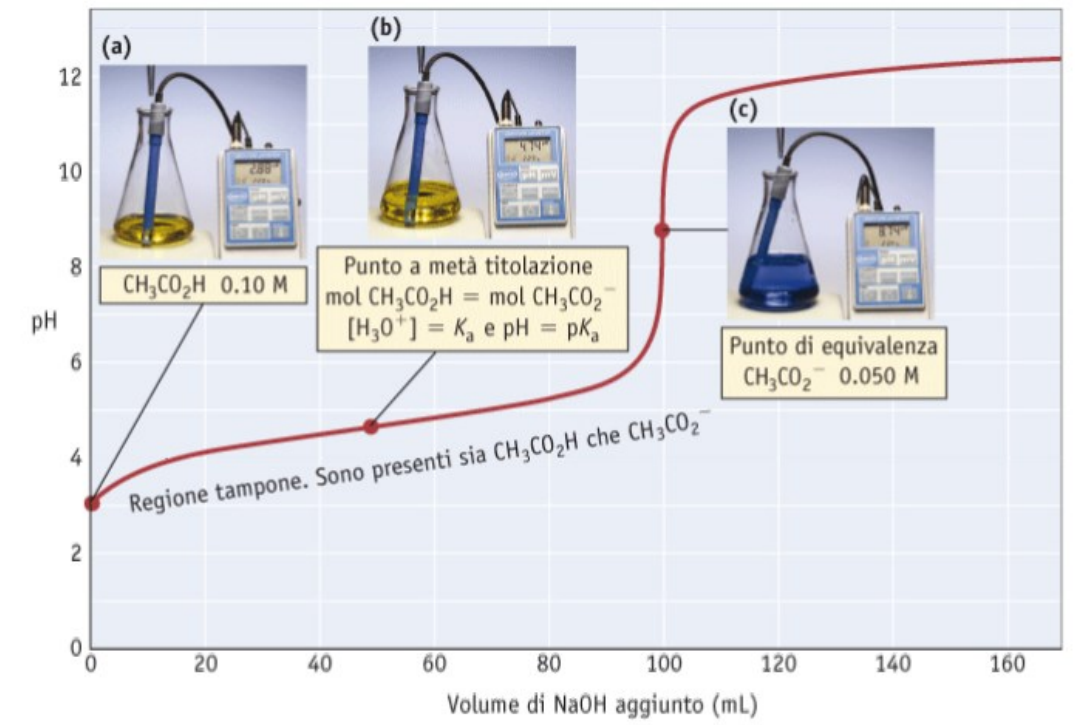
\includegraphics[width=14cm]{immagini/titolazione_acido_debole_base_forte.png}
\end{figure}

Molti saponi (pressoché tutti) in teoria sono neutri, così com'è neutra la polvere del cloruro di ammonio o dell'acetato di sodio, ma nell'istante in cui li mettiamo in acqua ci accorgiamo che il pH va in ambiente basico per casi come quello dell'acetato di sodio o in ambiente acido per casi come quello del cloruro di ammonio.

In questo caso, avendo acetato di sodio all'equivalenza il pH è superiore ad 8. Dopodiché con ulteriori aggiunte il pH si comporta come se fosse quello di una soluzione con base forte, cioè quando c'è l'eccesso di una specie forte è solo quella che va considerata.

\vspace{0.2cm}\textbf{Titolazione base debole-acido forte}

\vspace{0.2cm}Inizialmente abbiamo solo ammoniaca, che è una base debole, quindi il pH sarà basico. Se iniziamo ad aggiungere acido cloridrico il pH tenderà ad abbassarsi. Si forma così il tampone. Nell'istante in cui abbiamo neutralizzato il 50\% della base avremo il massimo potere tamponante.

Continuiamo ad aggiungere acido fino a neutralizzare tutta la base. Si forma il cloruro d'ammonio, che si dissocia in ammoniaca e ioni $\rm H_3O^+$, per cui l'ambiente diventa acido. Ne segue che all'equivalenza il pH sarà inferiore a 7: sarà 5.28\..

\begin{figure}[H]
    \centering
    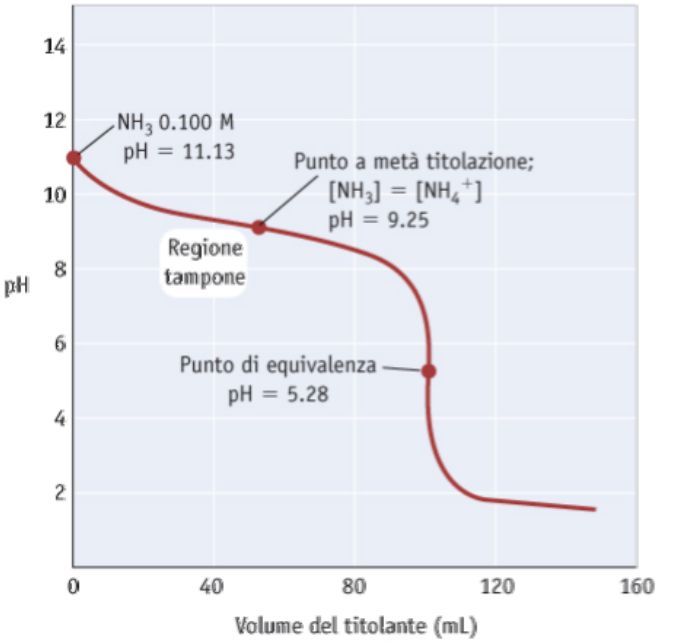
\includegraphics[width=10cm]{immagini/titolazione_base_debole_acido_forte.png}
\end{figure}

\subsection{Indicatori}
L'indicatore indica una variazione di pH. \E un composto che a seconda di come si dissocia mostra una forma acida e una forma basica aventi colori diversi.

Chiamiamo l'indicatore HIn\footnote{"In" non si riferisce all'elemento Indio, ma ad un elemento generico.}. \E una specie debole che si dissocia in $\rm H^+$ e $\rm In^-$ (ovviamente in acqua $\rm H^+$ si associa all'acqua dando $\rm H_3O^+$). Essendo una specie debole avremo una reazione di equilibrio di dissociazione e quindi una costante di equilibrio:

$$\ce{HIn(aq) + H_2O <--> H_3O^+ + In^-}$$

$$k_{In}=\frac{\rm{[H_3O^+]} \cdot \rm{[In^-]}}{\rm{[HIn]}}\implies \rm{[H_3O^+]}=\textit{k}_{\textit{In}} \frac{\rm{[HIn]}}{\rm{[In^-]}}$$

%Ogni ione $\rm H_3O^+$ corrisponderà ad uno ione $\rm In^-$, pertanto possiamo scrivere la concentrazione degli ioni $\rm H_3O^+$ al quadrato

$$\implies \rm pH = log \left( \frac{1}{[H_3O^+]} \right) = log \left( \frac{1}{\textit{k}_{\textit{In}}} \right) + log \left( \frac{\rm{[In^-]}}{\rm{[HIn]}} \right)$$

$$\implies \rm pH= p\textit{k}_\textit{a} + log \left( \frac{\rm{[In^-]}}{\rm{[HIn]}} \right)$$

Noi stiamo aggiungendo un colorante, che colora la soluzione in modo diverso a seconda che ci si trovi in ambiente acido o in ambiente basico. \E importante allora capire le quantità relative delle due forme colorate. Ad occhio nudo non riusciamo a vedere se uno dei due è in eccesso di un minimo: per vederlo è necessario che una delle due forme sia più abbondante dell'altra. Di norma allora si immagina di essere in condizioni tali che una delle due sia almeno 10 volte più abbondante dell'altra. Quindi potremmo avere uguali concentrazioni di $\rm In^-$ e HIn e in questo caso, se una forma è incolore e l'altra è colorata si percepisce la maggiore abbondanza di uno; se invece tutte e due le forme sono colorate in modo diverso (ad esempio in giallo e in blu) non è facile capire il colore della soluzione. Ne segue che quando si hanno le due forme entrambe colorate e in uguale concentrazione, sappiamo che il pH è uguale al p$k_a$, ma con i nostri occhi non siamo certi di percepire questo punto della titolazione.

Se invece $\rm [In^-]$ fosse 10 volte più grande di $\rm [HIn]$ il termine $\rm \log{\frac{[In^-]}{[HIn]}}$ dà 1; se $\rm [HIn]$ è 10 volte più grande di $\rm [In^-]$ il termine $\rm \log{\frac{[In^-]}{[HIn]}}$ dà -1:

\vspace{0.2cm}$\bullet \rm \; [In^-]=[HIn] \implies pH=p\textit{k}_{\textit{a}}$

\vspace{0.2cm}$\bullet \rm \; [In^-]=10[HIn] \implies pH=p\textit{k}_{\textit{a}}+1$

\vspace{0.2cm}$\bullet \rm \; [HIn]=10[In^-] \implies pH=p\textit{k}_{\textit{a}}-1$

\vspace{0.2cm}In questo modo ci mettiamo nelle condizioni di avere la preponderanza di uno o dell'altro con certezza senza che il pH vari drasticamente, in quanto sarà dato da p$k_a \pm 1$. Allora l'intervallo di viraggio varia da p$k_a - 1$ a p$k_a + 1$.

Notiamo che in prossimità del punto di viraggio queste variazioni avvengono con l'aggiunta di una sola goccia.

In questo modo anche se l'intervallo di viraggio è ampio non sbagliamo la titolazione. L'importante è andare a prendere l'indicatore che varia più o meno all'equivalenza.

\subsection{Solubilità}
Quando mettiamo qualcosa in acqua non è detto che essa si sciolga del tutto. Dobbiamo quindi stare attenti a ragionare su soluzioni, non sospensioni. In altre parole, se abbiamo messo in acqua un qualunque composto chimico e non si è sciolto totalmente, dobbiamo filtrare la soluzione. Ciò che non si è sciolto resterà nel filtro, la soluzione limpida invece passerà dal filtro e la otterremo nel becher.

\E quindi importante capire che esiste una \textbf{solubilità} di ogni specie chimica, la quale varia da composto a composto, passando da qualche milligrammo per litro a quasi un chilogrammo per litro.

Esempi di ciò sono il nitrato di potassio e il solfuro di mercurio. Della prima specie a 100° C se ne sciolgono circa 850 grammi in un litro di soluzione, mentre la seconda è talmente insolubile che forse in soluzione si scioglie qualche molecola.

\E possibile scrivere degli equilibri di solubilità per tutte le specie, ma non li tratteremo.